\documentclass[10pt,t]{beamer} % handout
\usetheme{Heverlee}
\usepackage{amsmath, amssymb}
\usepackage{mathtools}
\usepackage{tikz}
\usepackage{tikz-cd}
\usepackage{mathbbol}
\usepackage{subcaption}
\newtheorem{result}{Result}

% environments
%\newtheorem{theorem}{Theorem}
%\newtheorem{proposition}[theorem]{Proposition}
%\newtheorem{lemma}[theorem]{Lemma}
%\newtheorem{corollary}[theorem]{Corollary}
%\theoremstyle{definition}
%\newtheorem{definition}[theorem]{Definition}
%\newtheorem{example}[theorem]{Example}
%\newtheorem{remark}[theorem]{Remark}

% hyphenation
\hyphenation{co-chain}

% elements
\newcommand{\id}{\mathsf{id}}
\newcommand{\M}{\cM}
\newcommand{\UM}{{\forget(\M)}}
\newcommand{\SL}{{\M_{sl}}}
\newcommand{\USL}{{\forget(\M_{sl})}}
\newcommand{\Surj}{\cX}
\newcommand{\BE}{\cE}

% sets and spaces
\newcommand{\N}{\mathbb{N}}
\newcommand{\Z}{\mathbb{Z}}
\newcommand{\R}{\mathbb{R}}
\renewcommand{\k}{\Bbbk}
\renewcommand{\S}{\mathbb{S}}
\newcommand{\Ftwo}{{\mathbb{F}_2}}
\newcommand{\Fp}{{\mathbb{F}_p}}
\newcommand{\Cp}{{\mathbb{C}_p}}
\newcommand{\graphs}{\mathfrak{G}}
\newcommand{\gsimplex}{\mathbb{\Delta}}
\newcommand{\gcube}{\mathbb{I}}
\newcommand{\scube}[1]{(\triangle^{\!1})^{\times #1}}

% categories
\newcommand{\Cat}{\mathsf{Cat}}
\newcommand{\Fun}{\mathsf{Fun}}
\newcommand{\Set}{\mathsf{Set}}
\newcommand{\Top}{\mathsf{Top}}
\newcommand{\Ch}{\mathsf{Ch}}
\newcommand{\simplex}{\triangle}
\newcommand{\sSet}{\mathsf{sSet}}
\newcommand{\cube}{\square}
\newcommand{\cSet}{\mathsf{cSet}}
\newcommand{\Alg}{\mathsf{Alg}}
\newcommand{\coAlg}{\mathsf{coAlg}}
\newcommand{\biAlg}{\mathsf{biAlg}}
\newcommand{\sGrp}{\mathsf{sGrp}}
\newcommand{\Nec}{\mathsf{Nec}}
\newcommand{\nSet}{\mathsf{nSet}}
\newcommand{\Mon}{\mathsf{Mon}}
\newcommand{\Smod}{\mathsf{Mod}_{\S}}
\newcommand{\Sbimod}{\mathsf{biMod}_{\S}}
\newcommand{\operads}{\mathsf{Oper}}
\newcommand{\props}{\mathsf{Prop}}

% operators
\DeclareMathOperator{\free}{F}
\DeclareMathOperator{\forget}{U}
\DeclareMathOperator{\yoneda}{\mathcal{Y}}
\DeclareMathOperator{\chains}{N}
\DeclareMathOperator{\schains}{N^{\simplex}}
\DeclareMathOperator{\cchains}{N^{\cube}}
\DeclareMathOperator{\cochains}{N^{\vee}}
\DeclareMathOperator{\scochains}{N^{\vee}_{\simplex}}
\DeclareMathOperator{\ccochains}{N^{\vee}_{\cube}}
\DeclareMathOperator{\gchains}{C}
\DeclareMathOperator{\sSing}{Sing^{\simplex}}
\DeclareMathOperator{\cSing}{Sing^{\cube}}
\DeclareMathOperator{\loops}{\Omega}
\DeclareMathOperator{\cobar}{\mathbf{\Omega}}
\DeclareMathOperator{\triangulate}{\mathcal{T}}
\DeclareMathOperator{\cubify}{\mathcal{U}}
\DeclareMathOperator{\projection}{\pi}
\DeclareMathOperator{\inclusion}{\iota}

% other
\renewcommand{\th}{\mathrm{th}}
\newcommand{\op}{\mathrm{op}}
\DeclareMathOperator*{\colim}{colim}
\DeclareMathOperator{\coker}{coker}
\newcommand{\tensor}{\otimes}
\newcommand{\End}{\mathrm{End}}
\newcommand{\Hom}{\mathrm{Hom}}
\newcommand{\bars}[1]{\lvert#1\rvert}
\newcommand{\norm}[1]{\lVert#1\Vert}
\newcommand{\angles}[1]{\langle#1\rangle}
\newcommand{\pairing}[2]{\langle#1, #2\rangle}
\newcommand{\xla}[1]{\xleftarrow{#1}}
\newcommand{\xra}[1]{\xrightarrow{#1}}
\newcommand{\defeq}{\stackrel{\mathrm{def}}{=}}
\newcommand{\pdfEinfty}{\texorpdfstring{${E_\infty}$}{E-infty}}

% letters
\newcommand{\bC}{\mathbb{C}}

\newcommand{\cA}{\mathcal{A}}
\newcommand{\cB}{\mathcal{B}}
\newcommand{\cC}{\mathcal{C}}
\newcommand{\cD}{\mathcal{D}}
\newcommand{\cE}{\mathcal{E}}
\newcommand{\cM}{\mathcal{M}}
\newcommand{\cN}{\mathcal{N}}
\newcommand{\cO}{\mathcal{O}}
\newcommand{\cP}{\mathcal{P}}
\newcommand{\cW}{\mathcal{W}}
\newcommand{\cX}{\mathcal{X}}
\newcommand{\cY}{\mathcal{Y}}
\newcommand{\cZ}{\mathcal{Z}}

\newcommand{\rB}{\mathrm{B}}
\newcommand{\rE}{\mathrm{E}}
\newcommand{\rP}{\mathrm{P}}
\newcommand{\rR}{\mathrm{R}}

\newcommand{\sA}{\mathsf{A}}
\newcommand{\sB}{\mathsf{B}}
\newcommand{\sC}{\mathsf{C}}

% comments
\newcommand{\anibal}[1]{\textcolor{blue}{\underline{Anibal}: #1}}


\newcommand{\vk}{\vskip 5pt}
\newcommand{\press}{\textcolor{pblue}{PRESS}}

\newsavebox\precoproduct
\begin{lrbox}{\precoproduct}
	\begin{tikzpicture}[scale=.3]
	\draw (0,0)--(0,.8);
	\draw (0,0)--(.5,-.5);
	\draw (0,0)--(-.5,-.5);
	\end{tikzpicture}
\end{lrbox}
\newcommand{\coproduct}{% <- this 'right of' is inherited; how to avoid?
	\usebox\precoproduct}

\newsavebox\preproduct
\begin{lrbox}{\preproduct}
	\begin{tikzpicture}[scale=.3]
	\draw (0,0)--(0,-.8);
	\draw (0,0)--(.5,.5);
	\draw (0,0)--(-.5,.5);
	\end{tikzpicture}
\end{lrbox}
\newcommand{\product}{% <- this 'right of' is inherited; how to avoid?
	\usebox\preproduct}

%%% QUICK OPTIONS:
% (A) Math font without serifs, enable line below to make math serif:
    \usefonttheme[onlymath]{serif}

% (B) Re-define primary colour by adjusting the RGB values
    %\definecolor{pblue}{RGB}{206,125,66}

% (C) Title page graphic (optional) --- this is not for the background image, see \usebackgroundtemplate to change that ---
    %\titlegraphic{\includegraphics[height=2.7cm]{example_figure.pdf}}

% (D) Add logo to bottom right-corner (optional)
    \logo{\includegraphics[height=0.7cm]{aux/icosahedron-src.pdf}\hspace{12pt}\vspace{-6pt}}

% (E) Choose one (or none) of these lines to add footline bar on all frames
    %\setbeamertemplate{footline}[infoline]  % author, title, insitute
    %\setbeamertemplate{footline}[navigation] % dots swhowing progress
    %\setbeamertemplate{footline}[navsym] % navigation symbols

% (F) Widescreen 16:9 ratio
    %\usepackage[orientation=landscape,size=custom,width=16,height=9,scale=0.45,debug]{beamerposter}

%%% TITLE PAGE INFO:

\title{Effective constructions in algebraic topology}
\subtitle{with applications to machine learning and information theory}
\author[ammedmar]{Anibal M. Medina-Mardones}
\institute{Max Planck Institute for Mathematics in Bonn}
\date{August 2021}

\begin{document}
	%!TEX root = ../bugcat21.tex

{
	\usebackgroundtemplate{ \parbox[b][\paperheight][b]{\paperwidth}{\centering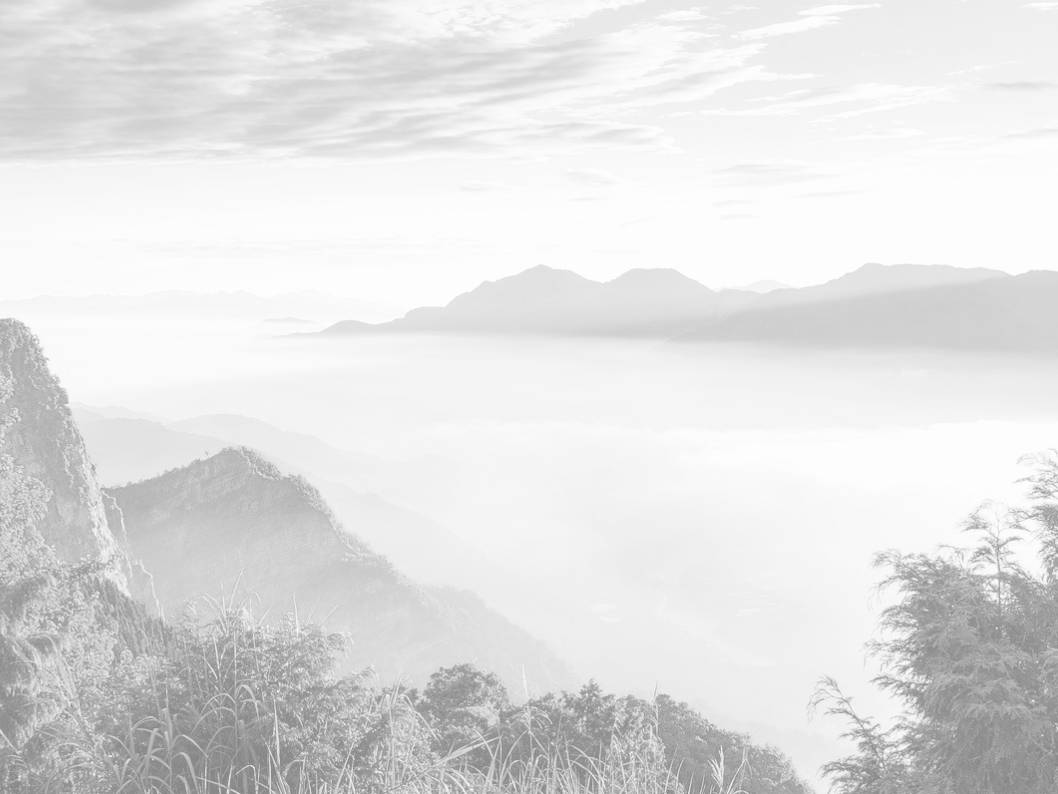
\includegraphics[width=\paperwidth]{aux/background.jpg}}}

	\setbeamercolor{background canvas}{bg=lgray}  % make background light gray

	\begin{frame}[plain,noframenumbering]
	    \titlepage
	\end{frame}
}
	%!TEX root = ../munich21.tex

\begin{frame}{Viewpoint}
	\vskip -10pt
	\begin{block}{A primary goal of algebraic topology}
		To construct invariants of topological space up to some notion of equivalence by recasting into combinatorial and algebraic models.
	\end{block}

	\medskip \pause
	\begin{block}{A basic tension}
		Computability vs. strength of invariants.
	\end{block}

	\medskip \textcolor{pblue}{Example:}
	Homology vs. homotopy.

	\medskip \pause
	\begin{block}{A more subtle tension}
		Effectiveness vs. functoriality of their constructions.
	\end{block}

	\medskip \textcolor{pblue}{Example:}
	cohomology via a cochain complex or \\
	\hspace*{40pt} via maps to Eilenberg-Maclane spaces.
\end{frame}

\begin{frame}{Modeling spaces combinatorially}
	\pause
	\begin{block}{Poincar\'{e}}
		Break spaces into contractible combinatorial pieces: simplices, cubes, ...
	\end{block}

	\pause \textcolor{pblue}{Cohomology:}
	via a cochain complex generated by these pieces.

	\medskip \pause	More generally:
	\begin{block}{Kan-Quillen}
		Use category theory to replace spaces by functors with a geometric realization: simplicial sets, cubical sets, ...
	\end{block}

	\pause \textcolor{pblue}{Basic objects:}
	Chains on standard pieces $\gchains(\gsimplex^n)$, $\gchains(\gcube^n)$, ...

	\smallskip \pause
	\begin{block}{Our goal (loosly stated)}
		Understand these chain complexes deeply to enhance (co)homology with finer effectively computable invariants.
	\end{block}
\end{frame}

\begin{frame}{Shortcomings of (co)homology}
	\pause With mod 2 coefficients the Torus and the Klein bottle are isomorphic
	\[
	H^\bullet(\mathsf T; \Ftwo) \cong H^\bullet(\mathsf K; \Ftwo)
	\]
	as graded vector spaces.

	\bigskip \pause
	Similarly,
	\[
	H^\bullet(\mathbb{C} P^2; \Z) \cong H^\bullet(S^2 \vee S^4; \Z)
	\]
	as graded abelian groups.

	\bigskip \pause
	\begin{block}{Cup product}
		These can be distinguished by the algebra/ring structure in cohomology.
	\end{block}
\end{frame}

\begin{frame}{Intersection intuition}
	\pause Cup product corresponds to intersection via Poincar\'e duality
	\pause
	\begin{figure}
		\newcommand*{\xMin}{0}%
\newcommand*{\xMax}{4}%
\newcommand*{\yMin}{0}%
\newcommand*{\yMax}{4}%
\begin{subfigure}{.4\textwidth}
	\centering
	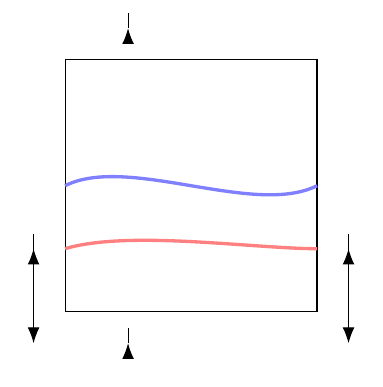
\begin{tikzpicture}[scale=.8]
	\draw[-{Latex[length=2mm]}] (-.5,\yMin)--(-.5,\yMax);
	\draw[-{Latex[length=2mm]}] (-.5,\yMin)--(-.5,\yMax-.5);
	\draw[-{Latex[length=2mm]}] (4.5,\yMin)--(4.5,\yMax);
	\draw[-{Latex[length=2mm]}] (4.5,\yMin)--(4.5,\yMax-.5);
	
	\draw[-{Latex[length=2mm]}] (\xMin, -.5)--(\xMax, -.5);
	\draw[-{Latex[length=2mm]}] (\xMin, 4.5)--(\xMax, 4.5);
	
	\draw (0,0)--(0,4)--(4,4)--(4,0)--(0,0);

	\draw[color=blue!50, very thick] (0,2) .. controls (1,2.5) and (3,1.5) .. (4,2);
	\draw[color=red!50, very thick] (0,1) .. controls (1,1.3) and (3,1) .. (4,1);
	\end{tikzpicture}
	\caption{Torus}
\end{subfigure}
\quad  
\begin{subfigure}{.4\textwidth}
	\centering
	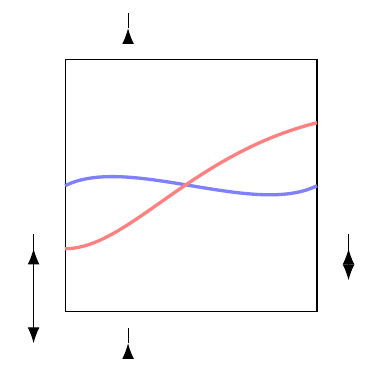
\begin{tikzpicture}[scale=.8]
	\draw[-{Latex[length=2mm]}] (-.5,\yMin)--(-.5,\yMax);
	\draw[-{Latex[length=2mm]}] (-.5,\yMin)--(-.5,\yMax-.5);
	\draw[-{Latex[length=2mm]}] (4.5,\yMax)--(4.5,\yMin);
	\draw[-{Latex[length=2mm]}] (4.5,\yMax)--(4.5,\yMin+.5);
	
	\draw[-{Latex[length=2mm]}] (\xMin, -.5)--(\xMax, -.5);
	\draw[-{Latex[length=2mm]}] (\xMin, 4.5)--(\xMax, 4.5);
	
	\draw (0,0)--(0,4)--(4,4)--(4,0)--(0,0);
		
	\draw[color=blue!50, very thick] (0,2) .. controls (1,2.5) and (3,1.5) .. (4,2);
	\draw[color=red!50, very thick] (0,1) .. controls (1,1) and (2,2.5) .. (4,3);
	\end{tikzpicture}
	\caption{Klein Bottle}
\end{subfigure}
		\label{f:torus and klein bottle}
	\end{figure}

	\textbf{Torus}: the (transverse) self-intersection for any 1-cycle is always \textcolor{pblue}{even}.

	\medskip

	\textbf{Klein Bottle}: the self-intersection of the depicted 1-cycle is \textcolor{pblue}{odd}.
\end{frame}
	%!TEX root = ../munich21.tex

\begin{frame}[fragile]{Cup product}
	\pause Alexander and Whitney defined the cup product by dualizing a chain approximation to the diagonal:
	\[
	\begin{split}
	\gchains(\gsimplex^n) &\to
	\gchains(\gsimplex^n) \otimes \gchains(\gsimplex^n) \\
	[v_0, \dots, v_m] &\mapsto
	\textstyle\sum_{i=1}^m \, [v_i, \dots, v_m] \otimes [v_i, \dots, v_m].
	\end{split}
	\]
	\pause Similarly, Cartan and Serre constructed: $\gchains(\gcube^n) \to \gchains(\gcube^n) \otimes \gchains(\gcube^n)$.

	\bigskip \pause
	As mentioned before, as graded rings,
	\[
	H^\bullet(\mathbb{C} P^2) \not\cong H^\bullet(S^2 \vee S^4).
	\]

	\vskip -8pt \pause But,
	\[
	H^\bullet(\Sigma(\mathbb{C} P^2)) \cong H^\bullet(\Sigma(S^2 \vee S^4)),
	\]
	where $\Sigma$ denotes suspension, for example $\Sigma(S^1)$ is
	\begin{center}
		\includegraphics[scale=.2]{aux/suspension.pdf}
	\end{center}
\end{frame}

\begin{frame}{Steenrod squares}
	\pause These chain approximations, unlike the diagonal of spaces, are \textcolor{pblue}{not} invariant under transposition: $x \otimes y \stackrel{T}{\mapsto} y \otimes x$.
	\begin{center}
		\begin{tikzpicture}
		\draw[color=pblue, thick] (0,0)--(1,1);
		\draw[->] (1.25, .5) -- (1.75, .5);
		\end{tikzpicture}
		\begin{tikzpicture}
		\node at (-0.1, 1){};
		\draw[color=pblue, thick] (0,0)--(1,0)--(1,1);
		\draw (1,1)--(0,1)--(0,0);
		\end{tikzpicture}
	\end{center}

	\medskip \pause To correct homotopically the breaking of this symmetry, Steenrod introduced explicit maps
	\[
	\Delta_i \colon \gchains(\gsimplex^n) \to \gchains(\gsimplex^n)^{\otimes 2},
	\qquad
	\partial \Delta_{i} = \big(1 \pm T \big) \Delta_{i-1}
	\]
	inducing further structure on mod 2 cohomology:
	\[
	\begin{split}
	Sq^k \colon H^\bullet(X; \Ftwo) &\to H^\bullet(X; \Ftwo) \\
	[\alpha] &\mapsto [(\alpha \otimes \alpha) \Delta_{k-|\alpha|}(-)]
	\end{split}
	\]
	\vskip -10pt \pause \textcolor{pblue}{Distinguishes}
	\[
	H^\bullet(\Sigma(\mathbb{C} P^2)) \not\cong H^\bullet(\Sigma(S^2 \vee S^4)).
	\]
\end{frame}

\begin{frame}[fragile]{A (new) description of Steenrod's construction}
	\pause \vskip -5pt \textcolor{pblue}{Notation:} \vspace*{-5pt}
	\[
	d_u[v_0, \dots, v_m] = [v_0, \dots, \widehat v_u, \dots, v_m]
	\]
	\pause \vspace*{-15pt}
	\[
	\rP_q(n) = \big\{ U \subseteq \{0,\dots,n\} : \bars{U} = q \big\}
	\]
	\pause \vspace*{-15pt}
	\[
	\forall \, U = \{u_1 < \dots < u_q\} \in \rP_q(n)
	\]
	\pause \vspace*{-15pt}
	\[
	d_U = d_{u_1} \dotsm \, d_{u_q}
	\]
	\pause \vspace*{-15pt}
	\[
	U^\varepsilon = \big\{ u_i \in U \mid u_i + i \equiv \varepsilon \text{ mod } 2 \big\}
	\]
	\pause \vskip -10pt
	\begin{definition}[Med.]
		For a basis element $x \in \gchains_m(\gsimplex^n)$
		\vspace*{-5pt}
		\[
		\Delta_i(x) \ = \!\!\! \sum_{U \in \rP_{m-i}(n)} \!\! d_{U^0}(x) \otimes d_{U^1}(x)
		\]
		\vspace*{-10pt}
	\end{definition}
	\pause \textcolor{pblue}{Example:} \vspace*{-5pt}
	\begin{align*}
	\Delta_0 [0,1,2] &=
	\Big( d_{12} \otimes \id + d_2 \otimes d_0 + \id \otimes d_{01} \Big) [0,1,2]^{\otimes 2} \\ &=
	[0] \otimes [0,1,2] + [0,1] \otimes [1,2] + [0,1,2] \otimes [2].
	\end{align*}
\end{frame}

\begin{frame}{Fast computation of Steenrod squares}
	\pause
	Comparing with SAGE: (algorithm based on EZ-AW contraction)

	\smallskip \pause
	\textcolor{pblue}{$Sq^1$} on \textcolor{pblue}{$\Sigma^i\R P^2$} ($i^\th$ suspension of the real projective plane)

	\medskip
	\includegraphics[width=\textwidth]{aux/comp_sus_rp2.pdf}
\end{frame}

	%!TEX root = ../munich21.tex

\begin{frame}{Point clouds}
	A data set can often be thought of as a point cloud in $\R^n$.

	\vskip 8pt

	Underlying probability distribution concentrated in a subspace.

	\vspace*{-5pt}

	\begin{center}
		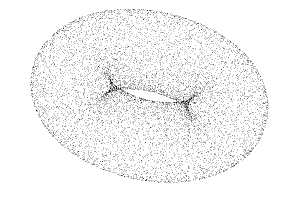
\includegraphics[scale=.3]{aux/torus}
	\end{center}

	\vspace*{-10pt} \pause

	How to approximate and study the underlying shape?

	\begin{center}
		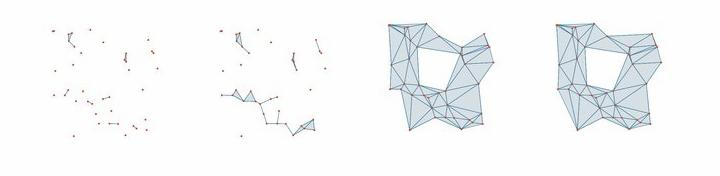
\includegraphics[scale=.4]{aux/filtration}
	\end{center}

	\vskip-15pt
	\textcolor{pblue}{Multi-scale approximation:} $X_1 \to X_2 \to \dots \to X_n$
\end{frame}

\begin{frame}{Persistence cohomology}

	\textcolor{pblue}{Barcode:}
	Quantifies ranks of all linear maps $H^n(X_j) \to H^n(X_i)$ for $i \leq j$.

	\pause
	\begin{center}
		\includegraphics[scale=.25]{aux/barcode.pdf}
	\end{center}

	\pause
	\textcolor{pblue}{Pipeline:}
	\begin{center}
		\includegraphics[scale=.8]{aux/diagram.pdf}
	\end{center}
\end{frame}

\begin{frame}[fragile]{Steenrod barcodes} \pause
	Given a filtered simplicial complex $X$
	\[
	X_0 \to X_1 \to \cdots \to X_n.
	\]
	\pause
	$Sq^k$ induces an endomorphism
	\[
	\begin{tikzcd}[column sep = small]
	H^\bullet(X_n; \Ftwo) \arrow[r] & \cdots \arrow[r] & H^\bullet(X_{n-1}; \Ftwo) \arrow[r] & H^\bullet(X_0; \Ftwo) \\
	H^\bullet(X_n; \Ftwo) \arrow[u, "Sq^k"] \arrow[r] & \cdots \arrow[r] & H^\bullet(X_{n-1}; \Ftwo) \arrow[u, "Sq^k"] \arrow[r] & H^\bullet(X_0; \Ftwo) \arrow[u, "Sq^k"].
	\end{tikzcd}
	\]
	The \textcolor{pblue}{$Sq^k$ barcode} of $X$ is the barcode of $\mathrm{img}\ Sq^k$.

	\bigskip \pause

	With \textit{Umberto Lupo} and \textit{Guillaume Tauzin} from \raisebox{-1pt}{
\includegraphics[scale=.1]{aux/giotto}}'s team

	\medskip
	develop a high-performance implementation: \textcolor{pblue}{\texttt{steenroder}}.
\end{frame}

\begin{frame}{Space of conformations of $\mathrm{C_8H_{16}}$}

	Points in $\R^{24}$ (positions of $8$ carbons in $\R^3$)

	\pause \smallskip

	Computing $Sq^1$ barcode of a ``smooth component'' of this point cloud

	\smallskip

	\includegraphics[width=\textwidth]{aux/cyclo-octane_subsampled_absolute_barcodes.pdf}

	Consistent with a \textcolor{pblue}{Klein bottle} component.
\end{frame}
	%!TEX root = ../munich21.tex

\begin{frame}[t]{Beyond the even prime}
	\pause

	Extending the diagonal to a full \textcolor{pblue}{$E_\infty$-coalgebra} structure on chains.

	\smallskip\pause

	These provide an algebraic model for the homotopy theory of spaces.\\ e.g. over $\mathbb Q$ (Quillen--Sullivan) over $\overline{\mathbb F}_p$ (Mandell).

	\smallskip\pause

	\begin{theorem}[Med.]
		The collection of maps $\gchains(\gsimplex^n) \to \gchains(\gsimplex^n)^{\otimes r}$ obtained from compositions of
		\begin{align*}
		\Delta &\colon \gchains(\gsimplex^n) \to \gchains(\gsimplex^n)^{\otimes 2}
		\qquad \text{(AW diagonal)} \\
		\ast &\colon \gchains(\gsimplex^n)^{\otimes 2} \to \gchains(\gsimplex^n)
		\qquad \text{(Join map)}
		\end{align*}
		defines an $E_\infty$-coalgebra on simplicial chains.
	\end{theorem}

	\pause \only<5>{\qquad \qquad \scalebox{0.7}{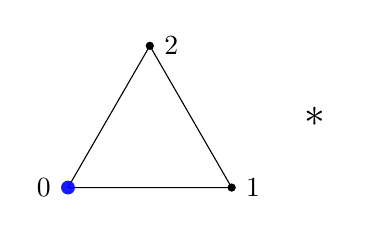
\begin{tikzpicture}[scale=.6]
\coordinate (A) at (210:2);
\coordinate (B) at (-30:2);
\coordinate (C) at (90:2);

\draw[draw=black] (A) -- (B) -- (C) -- (A);

\node[circle,fill=blue, opacity=.9, inner sep=0pt,minimum size=5pt, label=left:{0}] (a) at (A) {};
\node[circle,fill=black,inner sep=0pt,minimum size=3pt, label=right:{$1$}] (a) at (B) {};
\node[circle,fill=black,inner sep=0pt,minimum size=3pt, label=right:{$2$}] (a) at (C) {};

\node[scale=1.5] at (3.5,0.5) {$\ast$};
\end{tikzpicture}
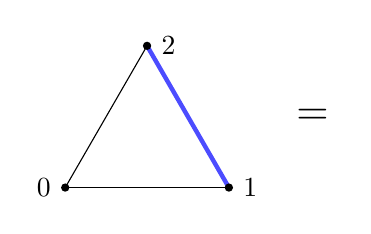
\begin{tikzpicture}[scale=.6]
\coordinate (A) at (210:2);
\coordinate (B) at (-30:2);
\coordinate (C) at (90:2);

\draw[draw=blue,  ultra thick, draw opacity=.7] (B) -- (C);
\draw[draw=black] (C) -- (A);
\draw[draw=black] (A) -- (B);

\node[circle,fill=black,inner sep=0pt,minimum size=3pt, label=left:{$0$}] (a) at (A) {};
\node[circle,fill=black,inner sep=0pt,minimum size=3pt, label=right:{$1$}] (a) at (B) {};
\node[circle,fill=black,inner sep=0pt,minimum size=3pt, label=right:{$2$}] (a) at (C) {};

\node[scale=1.5] at (3.5,.5) {=};
\end{tikzpicture}
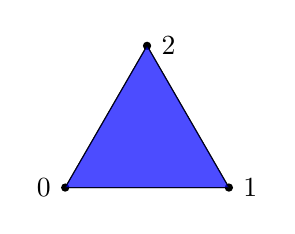
\begin{tikzpicture}[scale=.6]
\coordinate (A) at (210:2);
\coordinate (B) at (-30:2);
\coordinate (C) at (90:2);

\draw[draw=black] (A) -- (B) -- (C) -- (A);

\node[circle,fill=black,inner sep=0pt,minimum size=3pt, label=left:{$0$}] (a) at (A) {};
\node[circle,fill=black,inner sep=0pt,minimum size=3pt, label=right:{$1$}] (a) at (B) {};
\node[circle,fill=black,inner sep=0pt,minimum size=3pt, label=right:{$2$}] (a) at (C) {};

\draw[draw, fill=blue, opacity=.7] (A) -- (B) -- (C) -- (A);
\end{tikzpicture}}} \pause

	Used to introduce cup $(p,i)$-products effectively def. \textcolor{pblue}{Steenrod operations} on mod $p$ cohomology.
	\pause (Implemented in \texttt{comch}.)

	\smallskip\pause

	\only<8>{Also, versions for: \textcolor{pblue}{cubical} (R. Kaufmann) and
	\textcolor{pblue}{multisimplicial} chains (A. Pizzi \& P. Salvatore).}
\end{frame}

%	%!TEX root = ../munich21.tex

%\section{Even finer invariants}
\note{Let's discuss some even finer invariants of the cohomology of spaces}

\begin{frame}{Secondary operations}
	\note{Steenrod squares are defined by the cup-$i$ products which arise from lifting to the cochain level the commutativity relation of the cup product in cohomology. Recall, that the coboundary of cup-1 is the difference between cup-0 and its transpose.

	We are motivated then to look for other cohomological relations to lift.

	We look at Steenrod squares themselves, sometimes referred to as primary cohomology operations. They satisfy relations and the invariants that appear by lifting and solving these relations are known as secondary operations. \press

	There are two main relations that Steenrod squares satisfy: The Cartan and Adem relations. The first tells us how the squares interact with the cup product and the second tells us about their behaviour under interation. \press

	Can we lift these relations the cochain level?

	Yes, the cup-$i$ products can be used to define both, the squares and the cup product in cohomology, so we use them to express these relations in the form: cup-$i$ version of the left hand side minus cup-$i$ version of the right hand side equal to a coboundary \press

	So we wonder if we can solve these equation, effectively constructing such coboundaries, and unlocking secondary cohomology operations
}

	The $Sq^k$ are obtained from lifting the relation
	\begin{equation*}
	[\alpha] \smallsmile [\beta] = [\beta] \smallsmile [\alpha].
	\end{equation*}

	\pause

	What are \textcolor{pblue}{their} relations?
	\begin{align*}
	& Sq^k(\alpha \smallsmile \beta) = \sum_{i+j=k} Sq^i(\alpha) \smallsmile Sq^j(\beta), &&
	\text{(Cartan relation)} \\
	& Sq^i Sq^j(\alpha) = \sum_{k=0}^{\lfloor i/2 \rfloor} {j-k-1 \choose i-2k} Sq^{i+j-k} Sq^k(\alpha) &&
	\text{(Adem relation)}
	\end{align*}

	\pause
	\vskip 5pt
	\textcolor{pblue}{Can we lift these relations?} \pause
	Yes:
	\begin{equation*}
	C_k = \delta X, \qquad A_{i,j} = \delta Y,
	\end{equation*}
	\textcolor{pblue}{Can we solve them?}
\end{frame}

\begin{frame}[c]{Relations}

	\note{Another source of motivation for this question, and actually the original motivation for me, came from physicits studing exotic states of matter and other aspects of lattice field theory. \press

	Anton Kapustin from Caltech asked for a cochain level proof of the Cartan relation to have acces to these Cartan coboundaries, and they, together with Ryan Torngren now at Harvard, use some of my formulas in their work.

	\vk

	The question about Adem relations needed more ideas \press\
	and we tackle that project in collaboration with Greg Brumfiel from Stanford and John Morgan from Columbia.
}

	\pause

	\begin{result}[M-M]
		Effective construction of Cartan coboundaries.
	\end{result}

	Work motivated by physicist A. Kapustin (Caltech) and R. Thorngren (Harvard). They used my formulas in lattice field theory.

	\begin{center}
		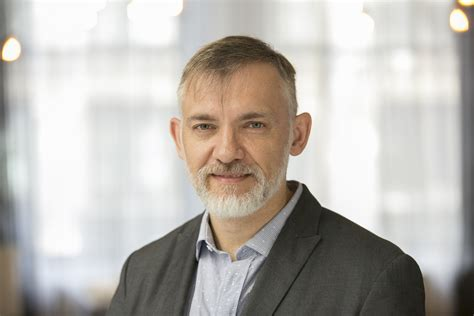
\includegraphics[scale=.13]{media/kapustin}
		\hspace*{1cm}
		
\includegraphics[scale=.21]{media/thorngren}
	\end{center}

	\pause
%	\vskip 20pt

	\begin{result}
		Effective construction of Adem coboundaries.
	\end{result}

	The above is joint with G. Brumfiel (Stanford) and J. Morgan (Columbia).

	\begin{center}
		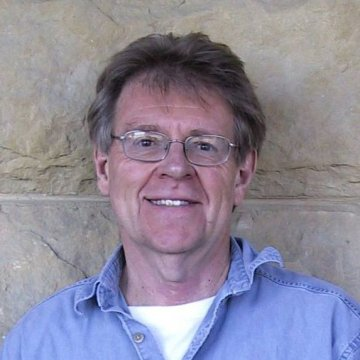
\includegraphics[scale=.21]{media/brumfiel}
		\hspace*{1cm}
		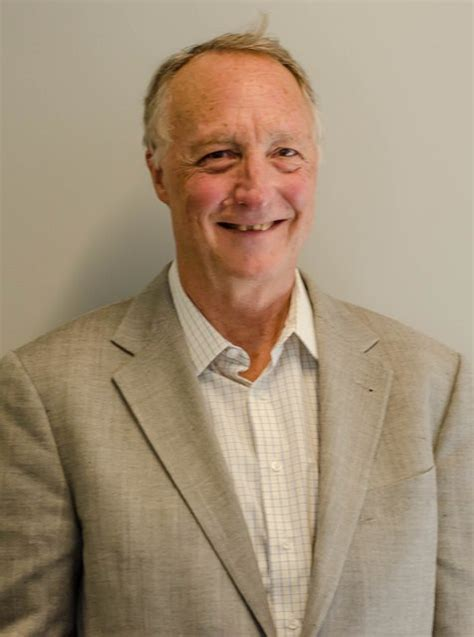
\includegraphics[scale=.09]{media/morgan}
	\end{center}
\end{frame}
	%!TEX root = ../bugcat21.tex

{
	\usebackgroundtemplate{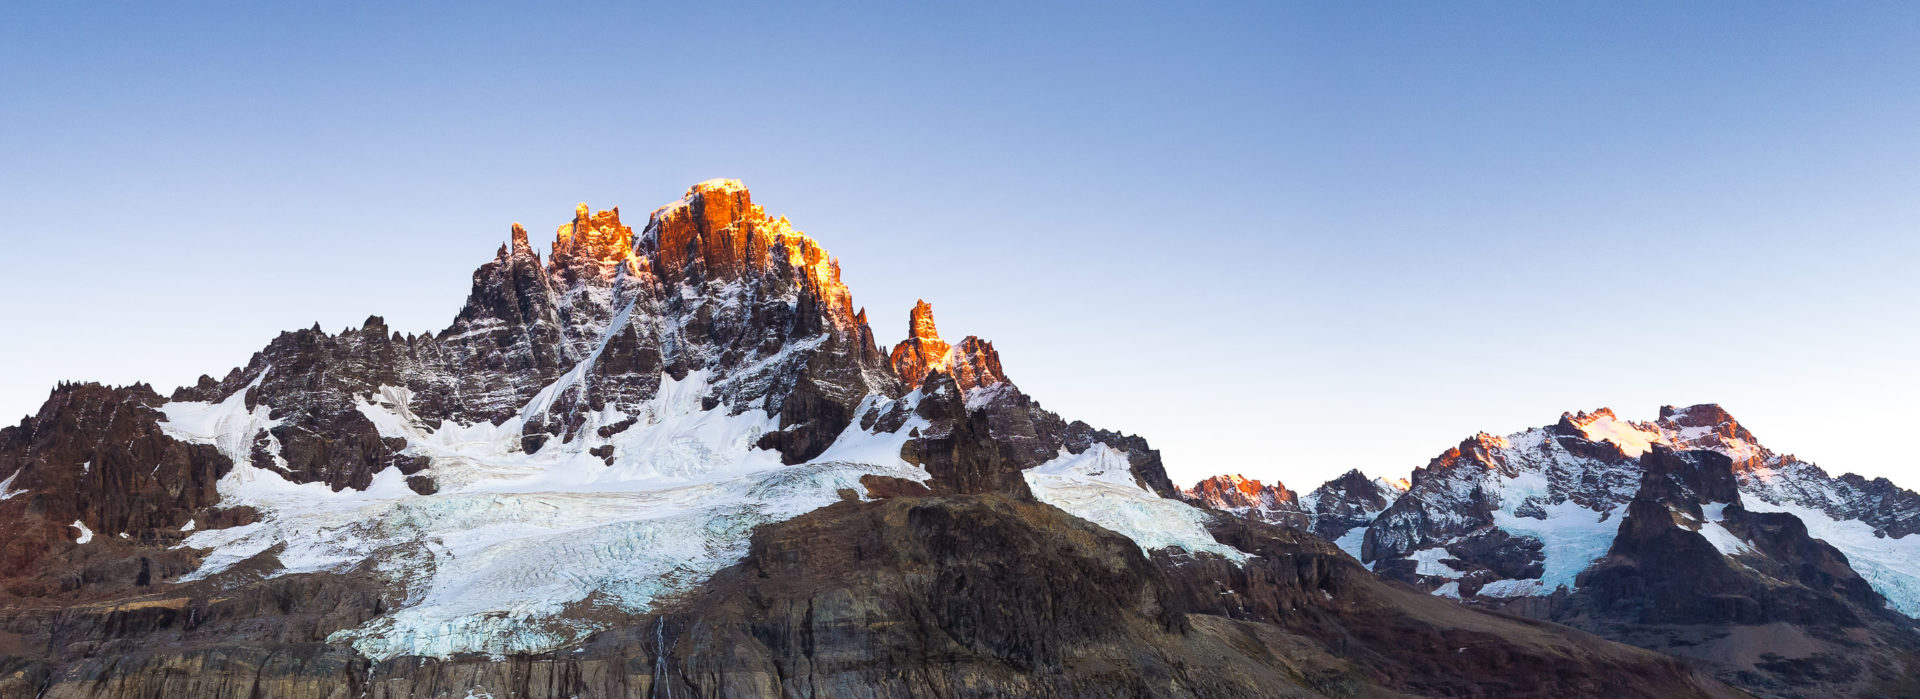
\includegraphics[width=\paperwidth]{aux/castillo.jpg}}%
	\begin{frame}
		\vskip 6cm
		\begin{center}
			\textcolor{pblue}{\Huge Thank you}
		\end{center}
	\end{frame}
}
	%!TEX root = ../munich21.tex

\begin{frame}{Graph Laplacian}

	\note{The graph Laplacian has become a primary tool for the study of networks.
	\vk
	It is typically defined using the incidence matrix of a graph and the valence matrix of its nodes, but we can equivalently define it using the boundary matrix that gave us 1-homology. \press

	Here is the definition and an example illustrating it.
	\vk
	Naturally, we can set $W$ to be the identity if we are interested in unweighted networks. \press

	The spectrum of this matrix is an important feature of the network. \press

	Additionally, we can consider the eigenvectors of the graph Laplacian. This preferred basis is often used for signal analysis on graphs. \press

	Where \textit{signal} in this context means a real-valued function from the set of vertices of the graph. \press

	What if we are interested in signals defined not just on vertices but on sets of such vertices? But even earlier, are there any interesting signals defined on subsets of vertices?
	}

	A powerful tool to study weighted networks.

	\vskip 5pt
	\pause

	\begin{center}
		\includegraphics[scale=.5]{media/graph}
	\end{center}

	\vskip -5pt

	\begin{equation*}
	\resizebox{8.5cm}{!}{
		$\partial_1 =
		\begin{pmatrix*}[r]
		-1 & -1 &  0 \\
		 1 &  0 & -1 \\
		 0 &  1 &  1
		\end{pmatrix*}
		\qquad
		W =
		\begin{pmatrix*}[r]
		w_{01}& 0      & 0 \\
		0     & w_{01} & 0 \\
		0     &      0 & w_{12}
		\end{pmatrix*}
		\qquad
		\partial_1^{\mathrm T} =
		\begin{pmatrix*}[r]
		-1 &  1 & 0 \\
		-1 &  0 & 1 \\
		 0 & -1 & 1
		\end{pmatrix*}$}
	\end{equation*}

	\vskip 10pt
	\pause

	Two types of uses:
	\begin{itemize}
		\item[] \textcolor{pblue}{Structural (eigenvalues).} The spectrum as a feature of the graph.

		\pause

		\item[] \textcolor{pblue}{Functional (eigenvectors).} A Fourier basis for signals on the graph, \\

		\vskip 5pt
		\hspace*{5cm} \pause i.e., real numbers at every node.
	\end{itemize}

	\pause

	What if the signals are defined \\
	\textcolor{pblue}{\ \ \ not just on single nodes?}
\end{frame}

\begin{frame}{Information signals}

	\note{In the study of complex systems it is often said that the whole is more than the sum of its parts. \press

	But how can we quantify this?

	After Shannon's ground-breaking work on information theory. We have a well developed framework that allows us to compute the information content shared by different parts of the system, treated as subspaces of a join probability distribution. \press

	For us is not so important to go over these definitions. It suffices to know they exist, and, therefore, that natural signals properly defined over simplices of high dimensions exist.

	For example, to an edge we can assign the mutual information shared by it vertices, for triangles, the interaction information of its vertices, and to higher dimensional simplices, we can assign appropriate generalizations of these. \press

	\vk

	A practical problem though, is the large number of simplices we get as we increase the number of vertices.

	\vk

	Maybe we can \textit{compress} this signals into a lower dimensional space?

	}

	\textcolor{pblue}{Complex Systems:} The whole is greater than the sum of its parts.

	\begin{center}
		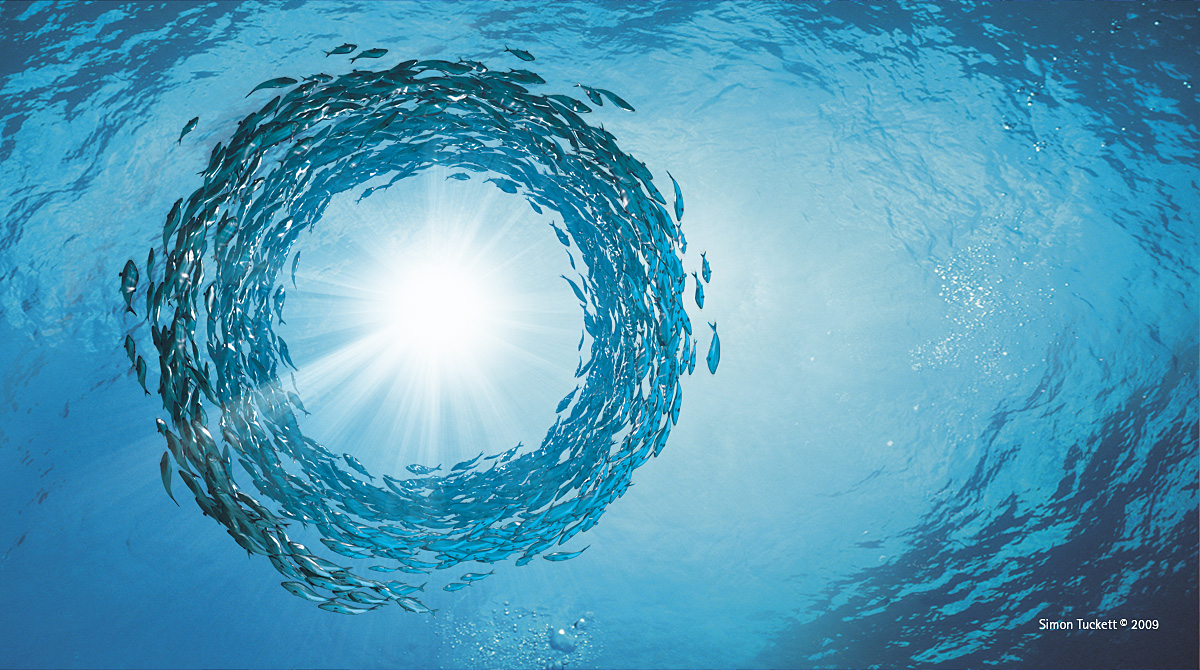
\includegraphics[scale=.12]{media/fishes}
	\end{center}

	\vskip 5pt
	\pause

	\textcolor{pblue}{But how to quantify this?}

	\vskip 5pt
	\pause

	Given collection of probability distributions $X_0, \dots, X_N$, can assign to

	\vskip 5pt

	\quad Pairs: their mutual information, \\
	\quad Triples: their interaction information, and\\
	\quad $(n+1)$-element sets: higher analogues of these.

	\vskip 5pt
	\pause

	\textcolor{pblue}{Problem:} The number of subsets grows exponentially with $N$.
\end{frame}

\begin{frame}{Hyperharmonic analysis}

	\note{Here is an analogy. Our cellphones are incapable of producing the fundamental frequency of most people's voices. But we still recognize them on the other side of the line, just hearing a lower fidelity version of their voices, that is, a lower dimensional representation of the signal. \press

	As another example, just a few harmonics are needed to distinguish a piano from a guitar playing the same note.

	Can we do something like that for information signals?

	Yes, indeed. \press

	Together with these researchers, we proposed a method that allows us to compress these signals substantially, reducing in this way some of the issues associated to the curse of dimensionality. \press

	As harmonic modes, we used the eigenvectors of a discrete analogue of the Laplace-de Rham operator of Riemannian geometry, which generalizes the graph Laplacian.

	And as a measure of compression, we use the cummulative explained variance, defined as follows. \press

	Consider a signal and a fix basis. Without loss of generality, order the coefficients of this signal, in that basis, so that their squares are non-increasing.
	The $k$-th explained variance is the proportion of the variance explained by the $k$-th coefficient, whereas the $k$-th cummulative explained variance is that explained by the first $k$ coefficients.
}

	\pause

	\vskip -5pt

	\textcolor{pblue}{Analogy:} We need only hear a few harmonics to distinguish a note played by a guitar or a piano.

	\vskip 5pt
	\pause

	\begin{result}
		Proposed a principled method to compress high-order information signals based on Fourier analysis and combinatorial topology.
	\end{result}

	Joint with F. Rosas (Imperial), S. Rodr\'iguez (UTFS) and R. Cofr\'e (PUCV).

	\vskip 15pt
	\pause

	\textcolor{pblue}{Discrete Laplacian:} $\displaystyle{L_n = \partial_{n+1} \partial_{n}^{\mathrm T} + \partial_{n-1}^{\mathrm T} \partial_{n}}$

	\vskip 15pt
	\pause

	\textcolor{pblue}{Compression:} $\alpha_1^2 \geq \alpha_2^2 \geq \cdots$ with $\{\alpha_i\}$ the coefficients in a basis.
	\begin{equation*}
	\text{EV}_{\alpha}(k) = \frac{ \alpha_k^2}{{\displaystyle \sum_{i} \alpha_i^2}}
	\qquad \text{ and } \qquad
	\text{CEV}_{\alpha}(k) = \sum_{1\leq i \leq k} \text{EV}_{\alpha}(i),
	\end{equation*}
\end{frame}

\begin{frame}{Proof of concept: Hadyn's symphonies}

	\note{\footnotesize
	As my last slide, let me show you some curves of the CEV obtained in a proof-of-concept example. \press

	We can think of a musical score as a multivariate time series, one time series for each instrument, and values between 0 and 12. This gives us a join probability distribution, based on the frequency of the notes.

	We considered the so called ``London symphonies" of Hadyn. \press

	And analysed two high-order generalization of Shannon's mutual information called O-information and S-information. These are proposed to respectively capture synergistic and redundant phenomena. Their interpretations will not play a role for us today, though.

	We computed them in dimension 2, 3, 4 and 5, corresponding to subsets of nodes of cardinalities between 3 and 6.

	And we then plotted the resulting CEV curves for the canonical basis and for the fourier basis. \press

	Here they are.

	\vk

	We can see that green and red reach high values very quickly. This tells us that with just a few coefficients in the fourier basis, we recover most of the signal. On the other hand, blue and orange require many more components to reach values close to 1, showing some of the advantges of the fourier basis over the canonical one, and based on a figure I am not showwing, also over randomly generated bases.

	\vk\vk
	--------------------


	Although, topology has been with mathematicians for over a century. In the past few years, we have seen an explosion of application of topology in the natural and computer sciences. And, thanks to the broader dissemination of \textit{its} ideas and the development of effective tools for its use, the insights that topology is providing researcher across diciplines are also... deepening.

	\vk

	With that said, I thank you very much for your time and attention.

}
	\vskip -5pt
	\pause

	Music as a probability distribution.

	\vskip 5pt
	\pause

	We analyzed two high-order information signals: O-info and S-info.

	\vskip 7pt
	\pause

	\hspace*{-15pt}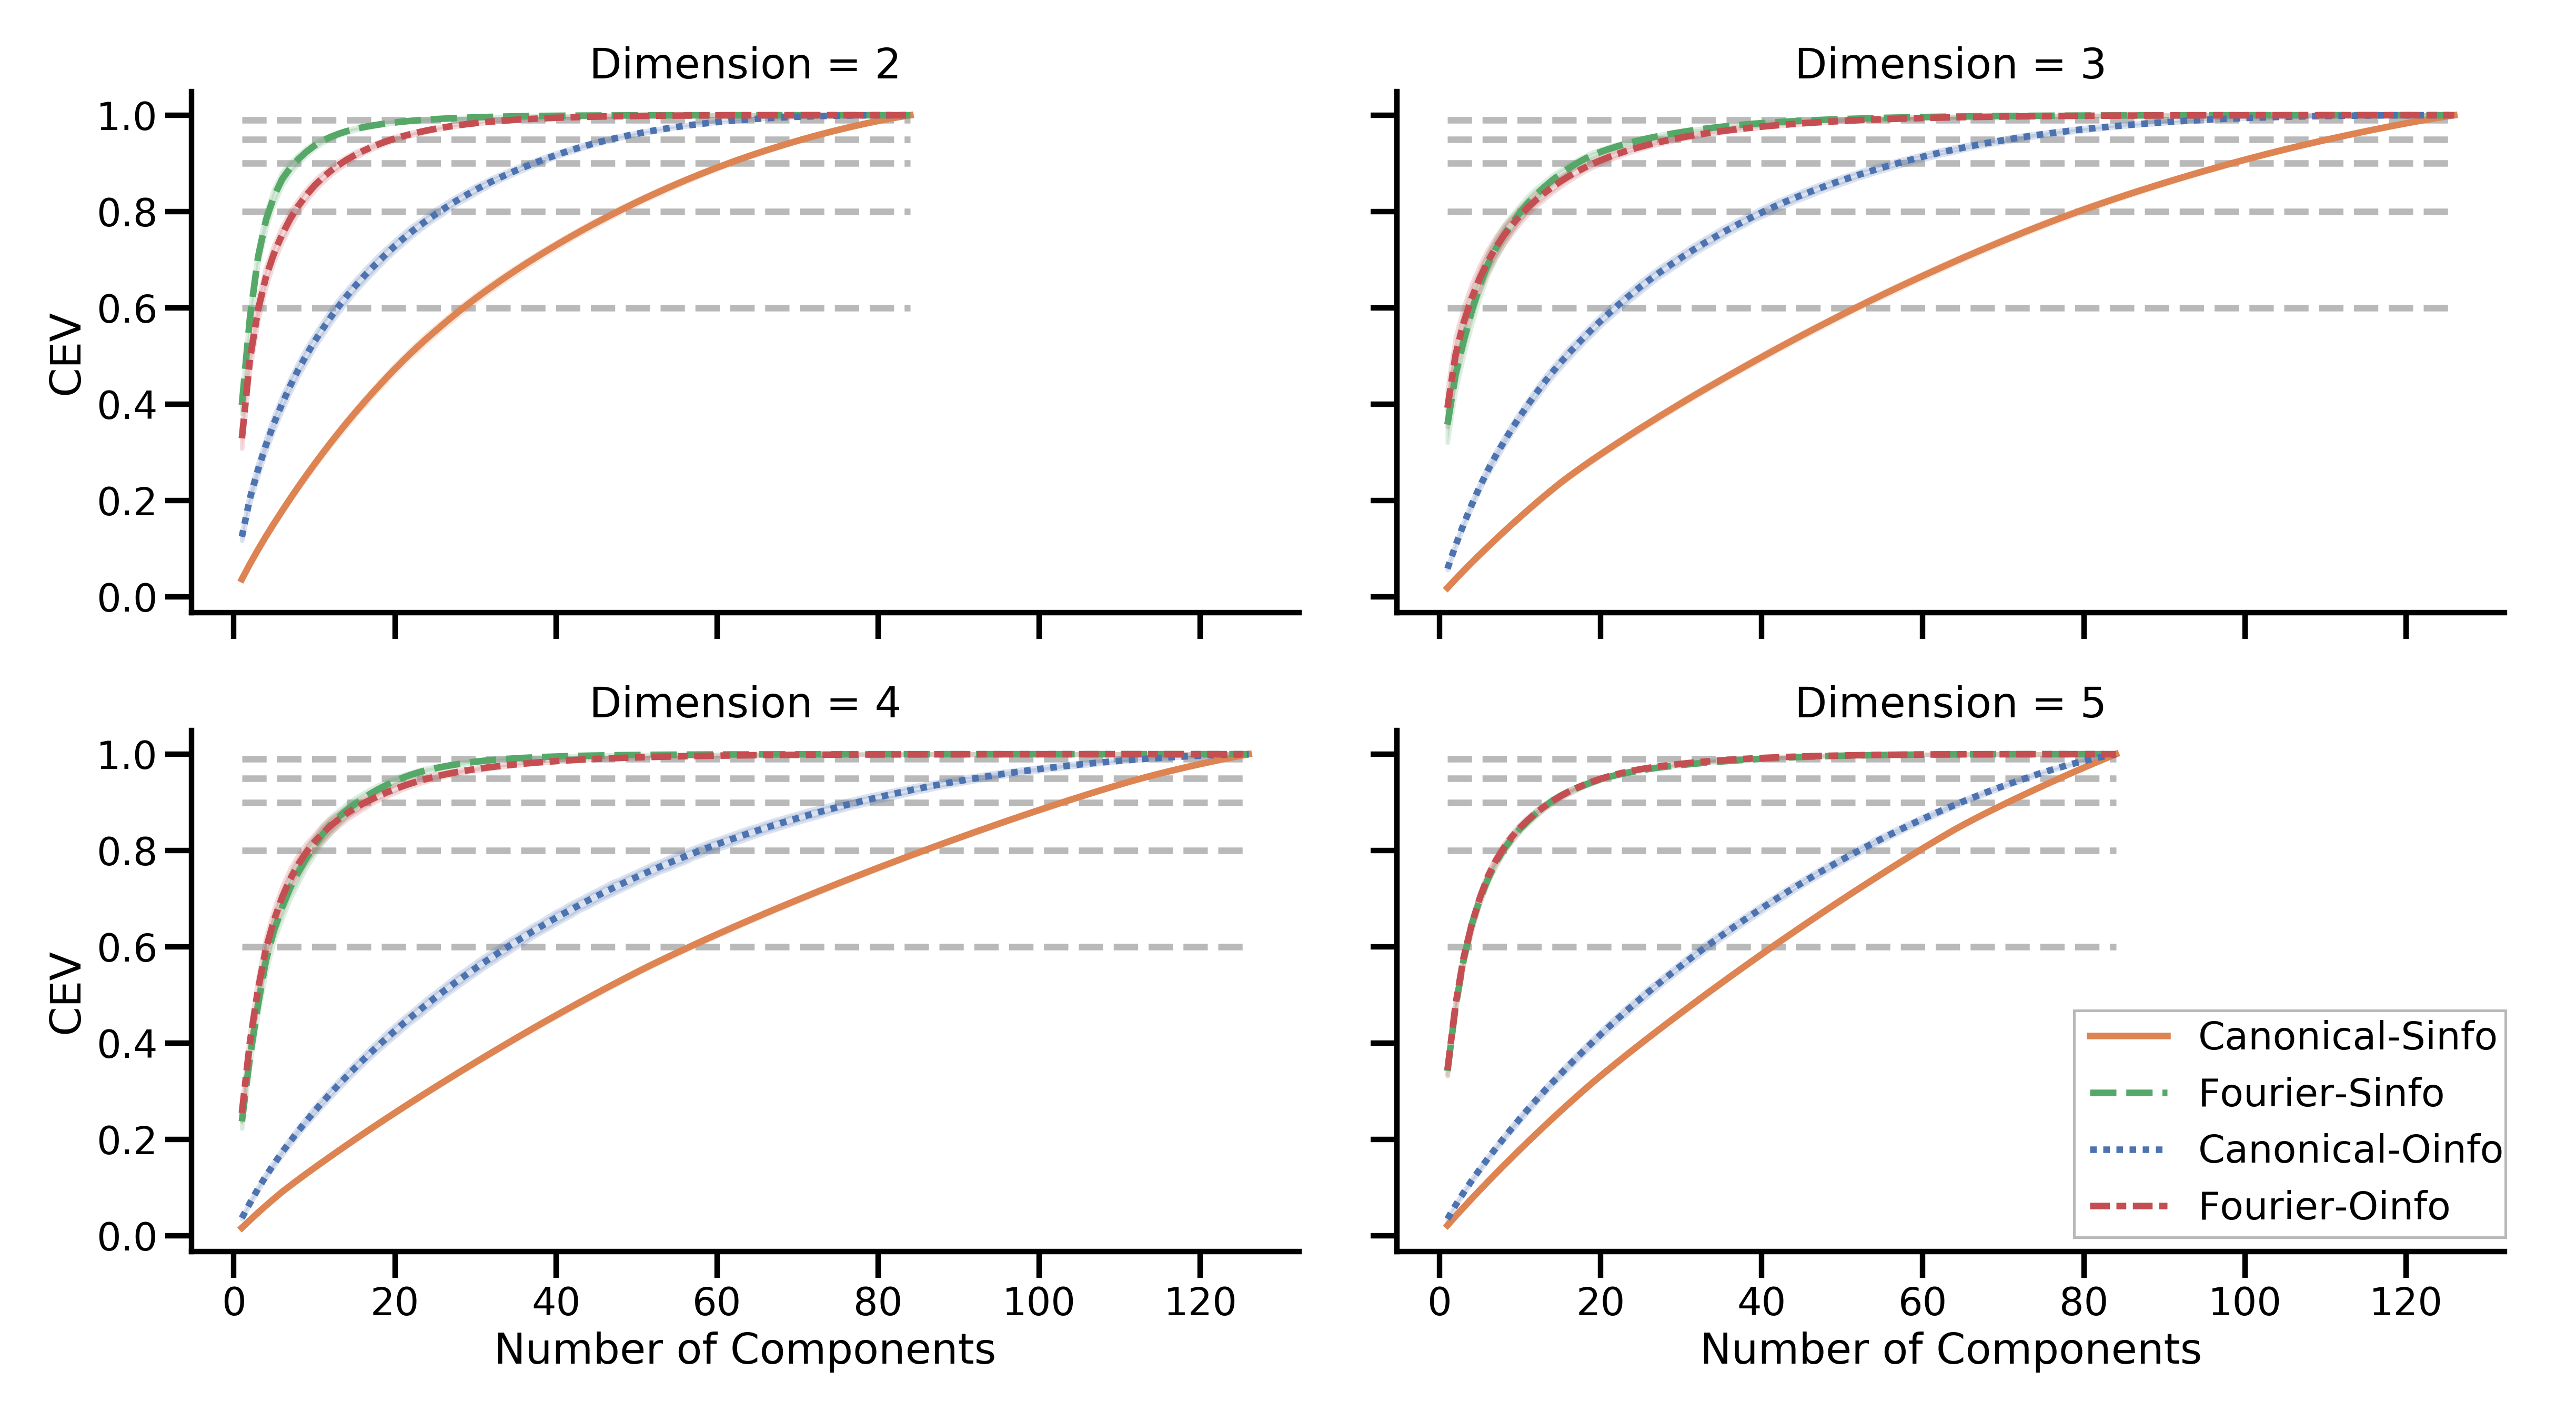
\includegraphics[scale=.096]{media/hyperharmonic}
\end{frame}
	%!TEX root = ../bugcat21.tex

{
	\usebackgroundtemplate{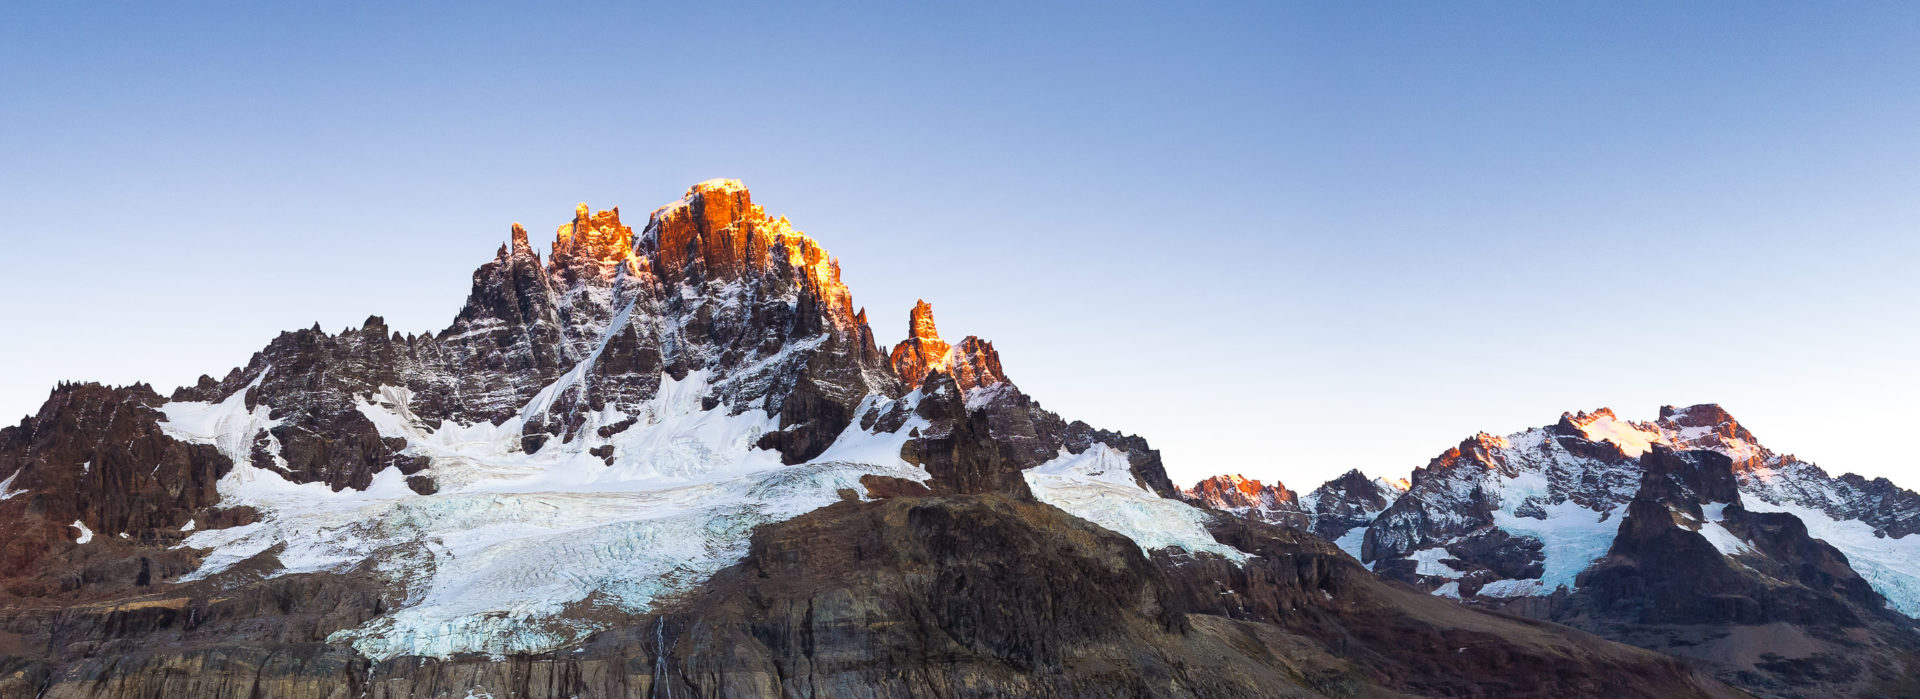
\includegraphics[width=\paperwidth]{aux/castillo.jpg}}%
	\begin{frame}
		\vskip 6cm
		\begin{center}
			\textcolor{pblue}{\Huge Thank you}
		\end{center}
	\end{frame}
}
\end{document}
